% Designed Companion Part IV figure
% Intended for \input{...} beside the matching canonical problem.
\begin{figure}[ht]
\centering
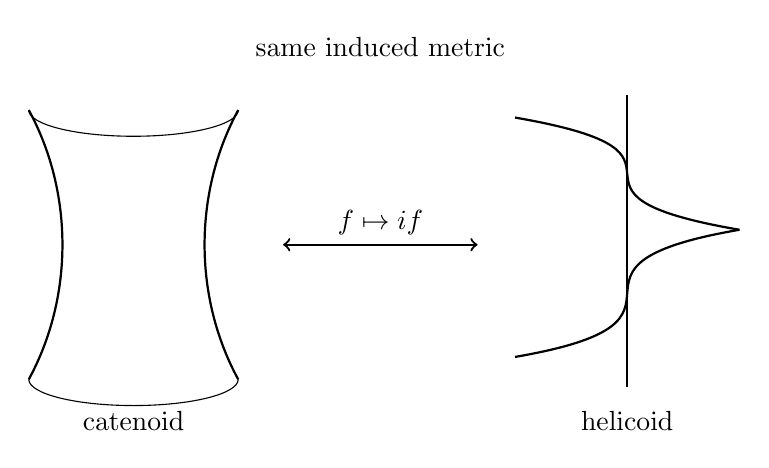
\begin{tikzpicture}[scale=0.95]
  \begin{scope}[xshift=-3.3cm]
    \draw[thick] (-1.4,-1.8) .. controls (-0.8,-0.7) and (-0.8,0.7) .. (-1.4,1.8);
    \draw[thick] (1.4,-1.8) .. controls (0.8,-0.7) and (0.8,0.7) .. (1.4,1.8);
    \draw (-1.4,-1.8) arc[start angle=180,end angle=360,x radius=1.4,y radius=0.35];
    \draw (-1.4,1.8) arc[start angle=180,end angle=360,x radius=1.4,y radius=0.35];
    \node at (0,-2.35) {catenoid};
  \end{scope}
  \draw[<->,thick] (-1.3,0)--(1.3,0) node[midway,above] {$f\mapsto if$};
  \begin{scope}[xshift=3.3cm]
    \draw[thick] (-1.5,-1.5) .. controls (1.4,-1.0) and (-1.4,-0.3) .. (1.5,0.2);
    \draw[thick] (1.5,0.2) .. controls (-1.4,0.7) and (1.4,1.2) .. (-1.5,1.7);
    \draw[thick] (0,-1.9)--(0,2.0);
    \node at (0,-2.35) {helicoid};
  \end{scope}
  \node at (0,2.65) {same induced metric};
\end{tikzpicture}
\caption{With the same Gauss-map data $g=e^z$, multiplying the Weierstrass function $f$ by $i$ moves from the catenoid to its associate helicoid. The associate pair is locally isometric.}
\label{fig:cp-iv-0060-catenoid-helicoid-associates}
\end{figure}
